\documentclass[8pt,a5paper]{acm_proc_article-sp}
% fix umlauts
\usepackage[ngerman]{babel}
\usepackage[utf8]{inputenc} 
\usepackage[T1]{fontenc}  % Times new Roman
\usepackage{mathptmx}
\usepackage[]{blindtext}
\usepackage[a5paper, left=1.70cm, right=1.20cm, top=1.30cm, bottom=1.40cm]{geometry}
\usepackage{epstopdf}
% balance columns. original from acm doesn't work
\usepackage{balance}
% colors
\usepackage[compact]{titlesec}
\usepackage{natbib}
\titlespacing{\section}{0pt}{*0.7}{*0.5}

\usepackage[nolist]{acronym}
 
\usepackage[usenames,dvipsnames]{xcolor}
% automatic crosslinks
\usepackage[colorlinks=true,citecolor=black,linkcolor=black,filecolor=black,urlcolor=black,pagebackref=true]{hyperref}
\hypersetup{colorlinks=true,citecolor=black,linkcolor=black,filecolor=black,urlcolor=black,pagebackref=true}
%glossaries
%\usepackage{makeidx}
%\makeindex
%\usepackage[nomain]{glossaries}
%\makeglossaries
%\makeindex

\newcommand{\glspl}[1]{{#1}}

% http://en.wikibooks.org/wiki/LaTeX/Glossary
% http://mirror.informatik.uni-mannheim.de/pub/mirrors/tex-archive/macros/latex/contrib/glossaries/glossariesbegin.pdf

% Definitionsliste
\newcommand{\defitem}[1]{\item[#1]\phantomsection\label{#1}\hfill\\} 
\newcommand{\defref}[1]{\hyperref[#1]{#1}} 
\newcommand{\rem}[1]{}
% Marking colors
\definecolor{todo}{rgb}{1,0.2,0.2}
\definecolor{reconsider}{rgb}{0.6,0.6,0.3}
\newcommand{\todo}[1]{{\color{todo} #1}}
\newcommand{\reconsider}[1]{{\color{reconsider} #1}}



\graphicspath{{img/}{./}}
\usepackage{graphicx}
\title{Portable System to Detect driver drowsiness with Body Sensors (PoSDBoS) \titlenote{ \scriptsize 
  \flushleft Betreuer Hochschule:  \ \ Prof. Dr. Martinez\\ 
  \qquad \qquad \qquad \qquad \quad \ \  Hochschule Reutlingen\\ 
  \qquad \quad \quad \quad \qquad \qquad \ \ Natividad.Martinez@Reutlingen-\\
  \qquad \qquad \qquad \qquad \quad \ \ University.de \\
  \includegraphics[width=1.8cm]{iot_hs_rt} \ \ \quad Master Project IoT 2016\\
  \ \ \\
  31. Juli 2016, Hochschule Reutlingen\\ 
  \copyright  ~ 2016 Paul Pasler}}


\numberofauthors{3}
\author{
	\alignauthor
	  \center
		\aufnt{Paul Pasler}\\
          \affaddr{Reutlingen University}\\
        \textbf{\textsf{Paul.Pasler@Student.Reutlingen-University.DE}}
}


\begin{document}
\begin{acronym}
\acro{FAS}{Fahrerassistenzsystem}
\acro{FASs}{Fahrerassistenzsysteme}
\acro{ME}{Müdigkeitserkennung}
\acro{MESs}{Müdigkeitserkennungssysteme}
\acro{ADAS}{Advanced Driver Assistance System}
\acro{ADASs}{Advanced Driver Assistance Systems}
\acro{bspw}{beispielsweise}
\acro{RTU}{Reutlingen University}
\acro{BS}{Körpersensoren}
\end{acronym}


\maketitle
\sloppypar{
\begin{abstract}
\acl{FASs} sind aus modernen Fahrzeugen nicht mehr wegzudenken. \acl{ME} hilft Sekundenschlaf oder müdigkeitsbedingte Unachtsamkeit zu vermeiden und verhindert somit schwere Unfälle. Systeme mit \acl{BS} zeigen in verschiedenen Studien sehr genau Ergebnisse und erkennen Müdigkeit frühzeitiger als andere Ansätze. In der vorgelegten Arbeit wurde ein solches System mit einem Elektroenzephalogramm (EEG) umgesetzt und getestet. Hierfür wurden Testdaten aufgenommen, verarbeitet und mit einem künstlichen Neuronalen Netz klassifiziert, sodass der aktuelle Status des Fahrers "`Wach"' oder "`Müde"' unterschieden werden kann.
\end{abstract}

\keywords{
\acl{FAS}, \acl{ME}, Elektroenzephalogramm, Signalverarbeitung, Machine Learning, Neuronales Netz
}

\category{A.0}{ACM}{
Experimentation
}


\section{Einleitung}
\label{chap:intro}
\acl{FASs} sind innerhalb weniger Jahren von der Oberklasse, in die Mittel-  und Kleinwagenklasse vorgedrungen. Die Unternehmensberatung Strategy Analytics schätzt, dass in den nächsten Jahren sechs mal soviele \acl{FASs} verbaut werden als heute \cite{strategy_analytics}. Sie bieten dem Fahrer erhöhten Komfort (Tempomat) oder die Sicherheit (Notbremsassistent). Laut der Boston Consulting Group, könnte der flächendeckende Einsatz von \acl{FASs}, die Unfallrate um ein knappes Drittel zurückgehen lassen \cite{bcgperspectives}. 

Zu Gruppe der Sicherheitsrelevanten \acl{FASs} gehört auch die \acl{ME}. Beispielsweise rät die \acl{ME} "`Attention Assist"' von Daimler dem Fahrer, zu gegebenen Anlass, eine Pause einzulegen und zeigt ein Kaffeesymbol im Cockpit an \cite{Daimler}. So wird müdigkeitsbedingte Unachtsamkeit oder Sekundenschlaf, die oftmals die Folge von schweren Unfälle sind, entgegengewirkt.

Neben überhöhter Geschwindigkeit, zählt laut dem Deutschen Verkehrssicherheitsrat Müdigkeit zu den häufigsten Unfallursachen und ist damit für jeden fünften schweren Unfall verantwortlich \cite{dvr_statistic}.  Dies verdeutlicht das Potential einer frühzeitigen Erkennung von Müdigkeit und einer Meldung an den Fahrer.


\begin{figure*} 
  \begin{center}
    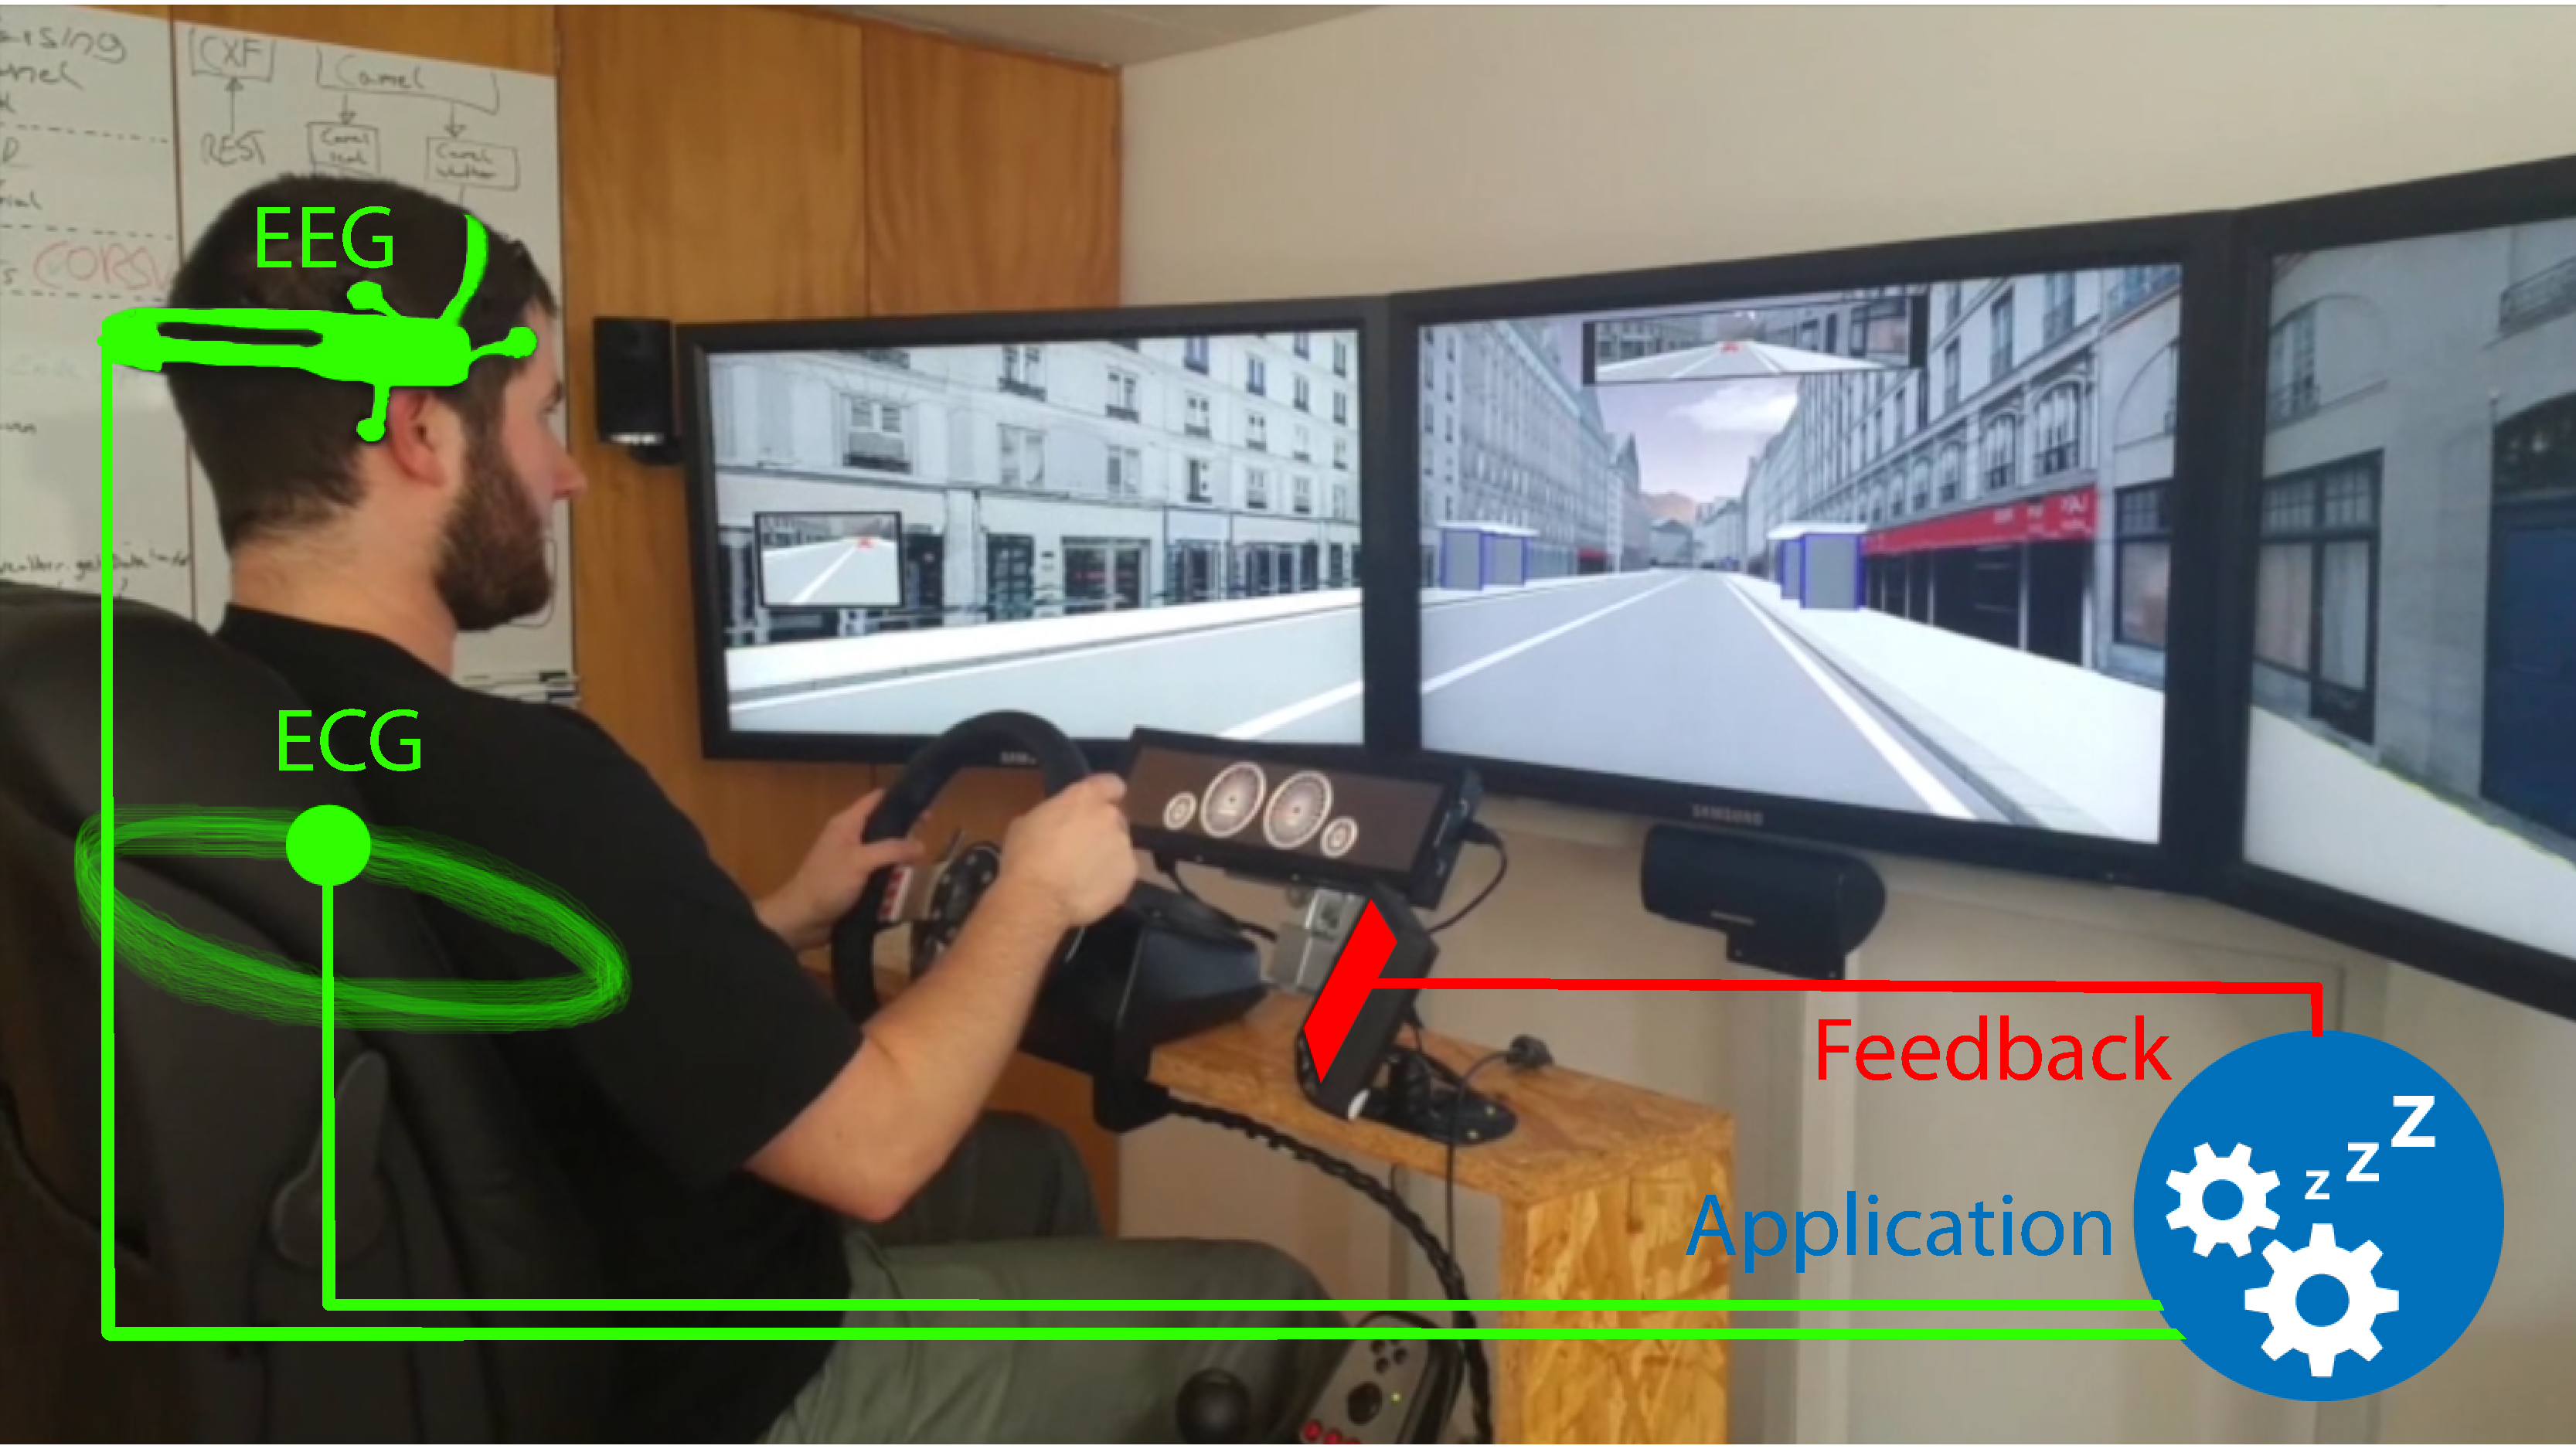
\includegraphics[width=12cm]{aufbau}
    \caption{Skizze des Systemaufbaus: \acl{BS} (Elektroenzephalografie / Elektrokardiogramm) liefert Daten an die Applikation und ein Feedback-Device warnt den müden Fahrer. Bild zeigt den Fahrsimulator der \acl{RTU}.}
    \label{fig:sketch}
  \end{center}
\end{figure*}

Um das Risiko eines Unfalls auf Grund von Übermüdung zu senken, soll langfristig ein multimodales System zu \acl{ME} entwickelt werden (Siehe Abb. \ref{fig:sketch}). Es existieren bereit diverse Systeme, denen es jedoch oftmals an Komfort und Portabilität mangelt. Ziel dieser Arbeit ist die Entwicklung eines Systems zur \acl{ME} mit einem EEG-Headset. 
Dessen Signale werden verarbeitet und mit einem KNN klassifiziert, mit dem Ziel den Fahrer rechtzeitig vor Übermüdung und deren Folgen zu warnen.
Statt dem klassischen EEG wird ein Emotiv Epoc eingesetzt werden, dadurch  soll die Beeinträchtigung des Fahrers möglichst gering gehalten
werden. Auch wenn sich der Ansatz weniger für den Serienbetrieb eignet, soll das System für die Validierung von berührungslosen Systemen verwendet werden. Die Notwendigen Testdaten werden im Rahmen des Projekts im Fahrsimulator der \acl{RTU} aufgenommen. Dennoch soll ganze System leicht portierbar sein, um es in einem echten Fahrzeug testen zu können.
\\ 

Die Ausarbeitung gliedert sich folgendermaßen. Im Kapitel \ref{chap:state} werden verschiedene Forschungsergebnisse zur \acl{ME} aufgezeigt und analysiert. Die Beschaffung der Daten und die durchgeführten Versuche sind  Thema von Kapitel \ref{chap:data}. Die Implementierung eines portablen Systems zur \acl{ME} mit \acl{BS} wird im Kapitel \ref{chap:implementation} vorgestellt. Kapitel \ref{chap:result} beschreibt die Ergebnisse und leitet in Kapitel \ref{chap:conclusion} zu den weiteren Schritten und dem Fazit über. In den anschließenden Absätzen werden Grundlagen für die kommenden Kapitel erläutert.

\section{Stand der Technik}
\label{chap:state}
Systeme zur Erkennung von Müdigkeit versuchen mit verschiedenen Parametern herauszufinden, ob sich die Person (der Fahrer) noch in einem aufmerksamen Zustand befindet. Die lässt sich in drei Bereiche unterteilen: Fahrverhalten, Computer-Vision (CV) und Körpersensoren. Die beiden ersten Bereich werden nur für die manuelle Markierung von Datensätzen genutzt. Die folgenden Ansätze beziehen sich ausschließlich auf die Erkennung mit Körpersensoren.

Für die Erkennung von Müdigkeit werden verschiedene Körpersensoren bzw. deren Kombination (multimodal) eingesetzt. Meist werden elektrische Spannung am und im Körper gemessen. 
Neben dem EEG, werden bspw. die Elektrokardiographie (EKG) oder Elektrookulografie (EOG) genutzt. Beim EKG wird die elektrische Aktivität des Herzmuskels erfasst, um bspw. die  Herzfrequenz zu bestimmen. Das EOG misst die Bewegung der Augen, um bspw. Blinzeln zu erkennen.

Ansätze mit einem EKG allein, zeigten in verschiedenen Arbeiten kein eindeutiges Ergebnis \cite{Vicente_6164509}, \cite{Rogado_4913155}. Beide versuchten Informationen aus der Herzfrequenzvariabilität zu erhalten und diese zu klassifizieren.

Khushaba et al. \cite{Khushaba_5580017} versuchten EEG, EKG und EOG zu verbinden und verglichen verschiedenen Kombinationen. Mit einem "`fuzzy wavlet"' basierten Algorithmus wurde die Signale aufbereitet und zeigten, dass ein EEG alleine bereits ausreicht. Die Kombination eines EEG mit EKG bzw. EOG verbesserte das Ergebnis nicht signifikant. Auch Johnson et. al \cite{Johnson11} kamen zu der Erkenntnis, dass ein EEG ausreicht und das genutzte EOG nicht benötigt wird. 

\cite{Subasi:2005:ARA:1707423.1707550} konnten mit einem EEG die Zustände "`Wach"', "`Schläfrig"' und "`Schlafend"' unterscheiden. Die Wavelet-Transformation und das genutzte künstliche Neuronale Netz (KNN) führten zu einer Erkennungsrate von 93\%. Vuckovic et al. fanden den besten Algorithmus für die Initialisierung des KNNs: Der Learning Vector Quantization Algorithmus. Im Vergleich mit EEG-Experten erreichte das KNN eine Übereinstimmung von 90\%. Huang et al. \cite{Huang_548971} nutzten ein Hidden Markov Modell zu Erkennung und erreichten eine gute Erfolgsrate.
Lin et al. \cite{Lin05eeg-baseddrowsiness} nutzten die Unabhängige Komponenten Analyse (UKA) und Lineare Regression (LR) und konnten zeigen, dass hiermit  bis zu 88\% richtige Ergebnisse erzielt werden können. 

Die betrachteten Arbeiten unterstreichen die Eignung des EEGs um Müdigkeit zu erkennen. Kombiniert mit anderen Sensoren können die Ergebnisse nur noch leicht verbessert werden.

\section{Datenbeschaffung}
\label{chap:data}
Um Daten von übermüdeten Fahrern zu erhalten, kann natürlich kein Versuch im Straßenverkehr durchgeführt werden. Die Fremd- und Eigengefährdung wäre einfach zu groß. Darum fanden die Versuche in einer Simulationsumgebung statt. Im Fahrsimulator der IoT Labs \footnote{\url{http://iotlab.reutlingen-university.de/}} der \acl{RTU} wird im Experiment eine Nacht-Autobahnfahrt simuliert. Verschiedene Studien \cite{Engstrom_2322937}, \cite{Horne_1757738} legen nahe, dass sich  Simulationen zwar von der Realität unterscheiden, dass jedoch die Ergebnisse trotzdem valide und brauchbar sind.

Der Fahrsimulator (Abb. \ref{fig:architecure}) besteht aus einem Simulationsrechner mit drei 20" Monitoren, einem echten Fahrersitz, Lenkrad, Schaltung und Pedalen. Für die Simulation wird die OpenSource Software "`OpenDS"' \footnote{\url{https://www.opends.eu}} genutzt. Per TCP/IP werden alle notwendigen Fahrzeugdaten vom Simulationsrechner auf den Datensammler und dort in ein virtuelles Steuergerät-Software (Vector CANoe \footnote{\url{https://vector.com/vi_canoe_de.html}}) geschickt. Über einen CAN-Bus können die Daten dann wieder, mittels einer Schnittstelle (CAN-Interface), ausgelesen werden. Die eigentliche Applikation wird auf dem Embeddedrechner ausgeführt.

\begin{figure}[h] 
  \begin{center}
    \includegraphics[width=6.5cm]{img/architecture}
    \caption[Aufbau des Simulators]{Der Aufbau des Simulators der \acl{RTU} mit den drei Rechnern für die Simulation, Datensammlung und Applikation. \label{fig:architecure}}
	
  \end{center}
\end{figure}

Für den Versuch werden neben den rohen EEG Signalen, auch die Fahrzeugdaten, sowie die Simulation und der Fahrer aufgenommen. Weiterhin kann der Versuchsleiter auch Besonderheiten protokollieren (Abb. \ref{fig:experiment}).

\begin{figure}[h] 
  \begin{center}
    \includegraphics[width=6.5cm]{img/experiment}
    \caption[Experiment]{Der Versuchsaufbau für die Erkennung von Müdigkeit mit den Datenströmen aus der Fahrerkabine zur Testüberwachung. \label{fig:experiment}}
  \end{center}
\end{figure}

Im Versuch sollte der Fahrer eindeutige Anzeichen von Müdigkeit zeigen. Dies kann durch verschiedene Versuchsparameter begünstigt werden. So zeigt eine Studie, dass Unfälle meist zwischen 2:00 - 6:00, sowie 14:00 - 16:00 Uhr passieren \cite{Horne_1757738}. Auch die Schlafmenge von weniger als 6 Stunden in der Nacht vor dem Experiment erhöht die Chance auf Anzeichen \cite{Engstrom_2322937}. Das Geschlecht oder Alter der Probanden ist nicht relevant. Vor dem Experiment sollten jedoch keine Drogen, Alkohol oder Kaffee eingenommen werden. Ein Führerschein ist von Vorteil, aber nicht zwingend notwendig.

Auch die Teststrecke (Abb. \ref{fig:drivingtask}) trägt zur Erhöhung der Müdigkeit bei. Monotone Autobahnfahrten die größtenteils geradeaus verlaufen, ohne andere Verkehrsteilnehmer und konstanter Geschwindigkeit führen eher zu einer Übermüdung. Nach diesen Kriterien wurde eine endlose zweispurige Autobahnkarte mit einer Geschwindigkeit von konstant 130Kmh erstellt. Sie spielt zudem Nachts und ist eher Dunkel gehalten, was besonders anstrengend für die Augen ist.

\begin{figure}[h] 
  \begin{center}
    \includegraphics[width=6cm]{img/drivingtask}
    \caption[Driving Task]{Die Autobahnkarte für den Versuch verläuft endlos geradeaus, Nachts und bei konstanter Geschwindigkeit. \label{fig:drivingtask}}
  \end{center}
\end{figure}

Für einen Versuch werden 40 Minuten angesetzt. Fünf Minuten werden für eine kurze Einführung, 30 Minuten für die Testfahrt und wieder fünf Minuten für eine kurze Einschätzung mit Fragebogen.

Anhand der aufgenommenen Daten werden nun Stellen gesucht, an denen die Testperson eindeutige Anzeichen von Müdigkeit zeigt. Eindeutig sind Verhaltensweisen wie häufiges Gähnen und Einnicken (Kopf fällt nach vorn) - Diese Merkmale werden häufig in CV-Ansätzen genutzt. 
Auch Verhaltensmerkmale wie, von der Spur abkommen und heftig Gegenlenken oder deutliche Veränderungen der Geschwindigkeit können Anzeichen für eine Unachtsamkeit wegen Müdigkeit sein.
Diese Stellen werden dann in den EEG Daten mit dem Label "`Müde"' markiert, alle anderen mit "`Wach"'. Die EEG Sequenzen können dann auf eindeutige Varianzen untersucht werden. Im nächsten Kapitel ist dies Thema der  Datenaufbereitung.



\section{Müdigkeitserkennung mit einem EEG-Headset}
\label{chap:implementation}

\section{Ergebnis}
\label{chap:result}

\section{Fazit und Ausblick}
\label{chap:conclusion}



\balance
\bibliographystyle{unsrt} % abbrv, alpha, plain, unsrt, apalike
\bibliography{Quellen}


\end{document}
